\documentclass[a4paper,12pt]{article}
\usepackage[utf8]{inputenc}
\usepackage[T1]{fontenc}
\usepackage{tipa}
\usepackage{graphicx}
\usepackage{rotating}
\usepackage{gb4n,lingsty, ipashortcuts}   
\usepackage{rotating}
\usepackage[authoryear]{natbib}
\bibpunct[:]{(}{)}{,}{a}{}{,}
\setlength{\bibsep}{0.05cm}
\newcommand{\ttrs}[2]{\parbox{3.5cm}{\em \textbf{#1} \em \\ `#2'}}
\newcommand{\nixbox}{\fbox{\parbox{2cm}{~ \\ ~}}}
%opening
\title{Sinhala influence in Sri Lanka Malay}
\author{Sebastian Nordhoff}
\date{ISMIL XIV 2010, Minneapolis}


\begin{document}
\let\eachwordone=\it
\let\eachwordtwo=\rm
\let\eachwordthree=\rm

\maketitle

\section{Introduction}
\begin{itemize}
 \item Sri Lanka Malay is a contact variety of  Malay which has undergone heavy grammatical restructuring towards Indian typology \citep{Smith2003timing, Paauw2004, SmithEtAl2004, SmithEtAl2006cll, Slomanson2006cll, Bakker2006, Ansaldo2008genesis, Nordhoff2009phd}
\item SOV word order, postpositions, preposed relative clauses, retroflexes
\item this restructuring is obviously due to contact with one or more local languages
\item candidate languages: Sinhala (Indo-Aryan) and Tamil (Dravidian)
\item opinions are divided on whether Tamil \citep{Smith2003timing, SmithEtAl2004} or Sinhala \citep{Ansaldo2008genesis} is the more important contact language
\item Sinhala is a good candidate because it is spoken by 4/5 of the population
\item Tamil is a good candidate because it is spoken by the ethnic group of the ``Moors'', who are Muslims just like the Malays.
\end{itemize}


\section{Question of origin}
\begin{itemize}
 \item In order to tell apart Sinhala influence from Tamil influence, one has to find areas where they differ.
\end{itemize}

\subsection{Smith's proposal}
\begin{itemize}
 \item Sinhala and Tamil are typologically very similar
 \item in many areas, SLM shows structures which are found in both Sinhala and Tamil
 \item for those cases, the source of a construction cannot be decided
 \item therefore: let's take a look at domains where Sinhala and Tamil diverge:
\begin{itemize}
 \item number marking
 \item accusative marking
 \item marking of (in)definiteness
\end{itemize}
 \item Influence in any of these domains can tip the scales in favour of either Sinhala or Tamil
\end{itemize}

\subsection{Smith's findings}
\begin{itemize}
 \item number marking
	\begin{itemize}
	\item Sinhala has obligatory number marking (sg/pl)
	\item Tamil has optional plural marking
	\item SLM has optional plural marking
	\item $\to$ Tamil influence
	\end{itemize}
 \item accusative marking
	\begin{itemize}
	\item Sinhala has only very marginal accusative marking
	\item Sinhala accusative can only be found on pronouns and animates
	\item Tamil accusative can be found on all pronouns and nouns
	\item SLM accusative can be found on all pronouns and nouns
	\item $\to$ Tamil influence
	\end{itemize}
\item marking of (in)definiteness
	\begin{itemize}
	 \item Sinhala has grammaticalized marking of indefiniteness
	 \item Tamil has no such marking
	 \item SLM has no such marking
	 \item $\to$ lack of Sinhala influence
	\end{itemize}
% \item retroflex stops
%  	\begin{itemize}
%  	 \item Tamil has retroflex stops in intervocalic position
% 	\item Sinhala has retroflex stops in initial and intervocalic position
% 	\item SLM has retroflex stops in intervocalic position
% 	\item $\to$ Tamil influence
%  	\end{itemize}
\item Smith's conclusion: at least three features of SLM point towards Tamil influence rather than Sinhala influence
\item explanation: heavy intermarriage between Tamil-speaking Moor women and Malay soldiers.
\item many Tamil speaking wives acquired the language of their Malay husbands, but only an imperfect version
\item this modified language was passed on to the children and spread through the generations
\item there were no Sinhala wives, so the absence of Sinhala influence is to be expected
\end{itemize}

\begin{itemize}
 \item I will challenge this scenario on both linguistic and sociohistorical grounds
	\begin{itemize}
	\item The claimed sociohistorical facts lack empirical evidence
	\item A closer look at Smith's domains reveals that there are actually more parallels with Sinhala than with Tamil
	\item this is corroborated by investigation of additional domains where Sinhala and Tamil diverge
	\end{itemize}
\end{itemize}

\section{Sociohistorical evidence}
\begin{itemize}
 \item This is discussed at length in \citet[40-47]{Nordhoff2009phd}
 \item It boils down to the fact that there is no hard and fast evidence for extensive intermarriage between Malays and Moors
 \item the relevant documents alluded to in \citet{Hussainmiya1987,Hussainmiya1990} are either lacking, or do not provide the necessary ethnographic information \citep{Ansaldo2008genesis}
\item lay genealogy compiled by \citet{Burah2006} points to exclusively Malay weddings in 62.4\% of the cases, plus 24.1\% which are either Malay or Moor
\item also early intermarriage with  Hindus, Burghers, and Sinhalese
\end{itemize}

\section{Review of Smith}
\subsection{Number marking}
\begin{itemize}
 \item Smith observes that number marking is obligatory in Sinhala, while it is optional in Tamil and SLM
 \item however, there is no need to invoke language contact here
 \item this feature seems to be a retention of the normal way to deal with number in Malay varieties
 \item number marking can simply not be used as a criterion to distinguish Tamil influence from Sinhala influence
 \item score: Sinhala 0; Tamil 0
\end{itemize}

\subsection{Accusative marking}
\begin{itemize}
 \item Smith claims that the SLM accusative marker aligns closely with the Tamil accusative marker
 \item the distribution of the Sinhala marker is argued to be different
 \item it is clear that the development of case is due to language contact
 \item however, Sinhala, Tamil and SLM actually have three different distributions of the accusative marker
\begin{itemize}
 \item Sinhala allows the accusative marker only on pronouns and animate nouns
 \item the Sinhala accusative is always optional, at least on nouns \citep[780]{Gair2003}
 \item Tamil allows the accusative marker on all nouns
 \item the accusative marker is obligatory on all definite objects and on all animate objects \citep[27]{Lehmann1989tamil}
 \item inanimate indefinite objects can lack the accusative marker under certain conditions \citep[27f]{Lehmann1989tamil}
 \item SLM accusative marking is optional, as in Sinhala, but shows a preference for referents which definite, topical, animate, affected, and singular \citep[329-332]{Nordhoff2009phd}
 \item The Tamil constraints against accusative marking on indefinite inanimates do not hold as the following example shows:


\xbox{\textwidth}{
 \ea\label{ex:form:yang:nottop:yang}
   \gll Derang \textbf{hathu}  papaaya=\textbf{yang}   asà-poothong \\
   \textsc{3pl} \textsc{indef} papaw=\textsc{acc} \textsc{cp}-cut  \\
`They cut a papaw' (K051220nar01)
\z
}

 \item The Tamil constraint to force accusative on animates does not hold either, as the following example shows 


\xbox{\textwidth}{
\ea \label{ex:form:yang:anim:notyang}
\gll Kumaareng=le      thuuju=so        dhlaapan=so        \textbf{oorang}=\zero{} asà-buunung. \\ % bf
     yesterday=\textsc{addit} seven=\textsc{undet} eight=\textsc{undet} man \textsc{cp}-kill  \\
    `Again yesterday, seven or eight people were killed.' (K051206nar11)
\z
} 

\end{itemize}
 \item this distribution seems to be a mix of Tamil and Sinhala constraints.
 \item score: Sinhala 0.5; Tamil 0.5
\end{itemize}

\subsection{Indefiniteness marking}
\begin{itemize}
 \item Smith claims that SLM lacks indefiniteness marking just like Tamil, but unlike Sinhala
 \item It is true that Tamil has no grammaticalized indefiniteness marking, while the Sinhala system is fully grammaticalized
\item \em Pace \em Smith, the claim that SLM lacks grammaticalized indefiniteness marking is empirically wrong
\item SLM has obligatory indefiniteness marking for
\begin{itemize}
 \item new referents
 \item predicates of class membership
 \item unspecific referents in general \citep[319-323]{Nordhoff2009phd}
\end{itemize}


\xbox{\textwidth}{
\ea \label{ex:hatthu:atthuhatthu}
\gll Se \textbf{atthu}=aade,  se \textbf{hatthu}=aade. \\
     \textsc{1s} \textsc{indef}=younger.sibling \textsc{1s} \textsc{indef}=younger.sibling  \\
    `I am a younger sibling, I am a younger sibling.'  (K061120nar01)
\z
}

\xbox{\textwidth}{
\ea \label{ex:hatthu:proclitic}
\gll \textbf{Hathu}=oorang=pe muuluth=dering \textbf{hathu}=criitha kal-dhaathang. \\
     \textsc{indef}=man=\textsc{poss} mouth=\textsc{abl} \textsc{indef}=story when-come  \\
    `When a story comes out of a man's mouth.'  (B060115prs15)
\z
}

\item this distribution mirrors exactly what we find in Sinhala
 \item additionally, the indefiniteness marker \em hatthu \em is also used with loanwords, whether they are indefinite or not
\item this is a clear calque of the Sinhala loanword integrator \em eka\em, orginally meaning `one'

\let\eachwordtwo=\it
\xbox{\textwidth}{
\ea \label{ex:hatthu:definite1}
\glll \textbf{Inni}     {\em mock}       {\em wedding}=\textbf{hatthu}  mas-gijja. \\
    Mee  {\em mock}       {\em wedding}=eka karan\dz a.oonä\\
      \textsc{prox} mock wedding=\textsc{indef}  must-make \\
    `I have to do this mock wedding.'  (K060116nar10)
\z
}
\let\eachwordtwo=\rm

\item in the domain of indefiniteness marking, SLM has clear parallels with Sinhala, and not with Tamil
\item score: Sinhala 1.5; Tamil 0.5
\end{itemize}


%
% \subsection{Retroflex stops}
% \begin{itemize}
%  \item Smith claims that SLM retroflex stops are only found intervocalically, just like Tamil retroflex stops, whereas Sinhala retroflex stops can also be found initially
% \item this makes Tamil influence more likely
% \item it is true that Tamil has a constraint against initial retroflex stops, which is not found in Sinhala
% \item however, SLM does not have this constraint either, there are many cases of initial retroflex \dz, e.g. \phontrs{\dz a:pa\dentt}{get}
% \item the distribution of retroflex stops thus points towards Sinhala influence, rather than Tamil influence
% \item score: Sinhala 2.5; Tamil 0.5
% \end{itemize}

\subsection{Intermediate conclusion}
\begin{itemize}
 \item Even with the domains chosen by Smith et al, we find more Sinhala influence than Tamil influence
 \item Let's take a look at more domains:
	\begin{itemize}
	 \item number of stop series
	 \item gemination
	 \item distribution of stops and nasals
	 \item modal particles
	 \item involitive derivation
	 \item dative and accusative subjects
	 \item zero adclausal nominalization
 	 \item adhortative construction
	\end{itemize}
\end{itemize}




\section{More features}
\begin{itemize}
 \item The following features were chosen because Sinhala and Tamil diverge there
\end{itemize}

\subsection{Number of stop series}
\begin{itemize}
 \item Most if not all Malay varieties have 2 series of stops: they contrast a series of voiceless stops (p,t,c,k) with a series of  voiced stops (b,d,j,g).
 \item Tamil has only 1 series (p, \dentt, (\textsubbar{r}), \tz, c, k), with voicing conditioned by phonotactics
 \item Sinhala has 3 series: voiceless (p, \dentt, \tz, c, k), voiced (b, \dentd, \dz, j, g), and prenasalized (\umb, \undentd, \undz,  \ung)
 \item SLM also has 3 series: voiceless (p, \dentt, \tz, c, k), voiced (b, \dentd, \dz, j, g), and prenasalized (\umb, \undentd, \undz, \unj, \ung)
\item the SLM stops look very much like the Sinhala stops (with the addition of \unj)
\item score: Sinhala 2.5; Tamil 0.5
\end{itemize}
%
% \begin{table}
% \centering
% \begin{tabular}{llll}
%
% schema & V\textsubring CV & V\textsubwedge CV & VNV \\
% %
% model & apa & aba & ama   \\\\
% %
% Malay & \ttrs{kapan}{when} & \ttrs{raba}{stroke} & \ttrs{sama}{all} \\\\
% %
% Tamil & \nixbox & \ttrs{tabaal}{mail} & \ttrs{aamaa}{yes} \\\\
% %
% Sinhala & \ttrs{epaa}{don't want} & \ttrs{babaa}{baby} & \ttrs{kamak}{difficulty} \\\\
% %
% SLM & \ttrs{kaapang}{when} & \ttrs{raaba}{stroke} & \ttrs{kaamar}{room} \\
%
% \end{tabular}
% \caption{Intervocalic stops}
% \end{table}


\subsection{gemination}
\begin{itemize}
 \item Most if not all varieties of Malay do not have gemination
 \item Tamil, Sinhala, and SLM have gemination
 \item gemination is thus a good candidate for language contact
 \item Tamil only has gemination of voiceless stops, and sonorants. There are no geminated voiced stops in Tamil
 \item Sinhala has gemination of voiceless stops, voiced stops, and sonorants
 \item SLM also has gemination of voiceless stops, voiced stops, and sonorants (Table \ref{tab:gemination})
 \item Sinhala and SLM are closely parallel
 \item score: Sinhala 3.5; Tamil 0.5
\end{itemize}


\begin{table}
\begin{tabular}{llll}

schema &    V\textsubring C\textsubring CV & V\textsubwedge C\textsubwedge CV & VNNV \\
%
model &  appa & abba & amma  \\\\
%
Malay  & \nixbox & \nixbox & \nixbox  \\\\
%
Tamil &  \ttrs{appaa}{father} & \nixbox & \ttrs{ammaa}{mother}  \\\\
%
Sinhala & \ttrs{baappaa}{uncle} & \ttrs{ibba}{tortoise} & \ttrs{ammaa}{mother} \\\\
%
SLM & \ttrs{kappal}{ship} & \ttrs{habbar}{news} & \ttrs{samma}{all} \\
\end{tabular}
\caption{Gemination}
\label{tab:gemination}
\end{table}


\subsection{Distribution of stops and nasals}
\begin{itemize}
 \item most varieties of Malay have two possible combinations of nasal+stop
	\begin{itemize}
	 \item `plain' varieties: [mp], [mb] (sampi, ambil)
 	 \item `prenasalizing' varieties: [mp], [$^m$b] (sampi, a$^m$bil)
	\end{itemize}
 \item Tamil only has [mb]
\item Sinhala has [mp], [mb] and [$^m$b]
\item SLM also has [mp], [mb] and [$^m$b] (Table \ref{tab:NC})
\item the distribution of stops and nasals is parallel between Sinhala and SLM
 \item score: Sinhala 4.5; Tamil 0.5
\end{itemize}



\begin{table}
\begin{tabular}{llll}
schema & VN\textsubring CV & VN\textsubwedge CV & V$^N$\textsubwedge CV \\
%
model & ampa & amba & a$^m$ba   \\\\
%
Malay &  \ttrs{rumput}{grass} & \multicolumn{2}{c}{\ttrs{$\leftarrow$sambal$\rightarrow$}{condiment}}\\\\
%
Tamil & \nixbox & \ttrs{ambadu}{50} &  \nixbox  \\\\
%
Sinhala & \ttrs{Gampaha}{(place name)} & \ttrs{kamba}{cloth book cover} & \ttrs{ka$^m$ba}{ropes} \\\\
%
SLM & \ttrs{kampak}{axe} & \ttrs{sambal}{condiment} & \ttrs{gaa$^m$bar}{picture} \\\\
\end{tabular}
\caption{Sequences of nasal+stop}
\label{tab:NC}
\end{table}


\subsection{modal particles}
\begin{itemize}
 \item modality is expressed in Malay varieties by particles like \em boleh \em
 \item Sinhala uses so called quasi-verbs with limited inflectional potential \citep{Gair1970}
 \item Tamil uses fossilized third person singular neuter future forms of a number of verbs \em  vee\nz um, poodum (, teriyum, mu\dz iyum)  \em etc. \citep[84]{Lehmann1989tamil}
 \item SLM has the particles \trs{boole}{can}, \trs{maau}{want},   and \trs{thussa}{not.want}, \em which seem to align more closely with Sinhala \em puluvan, oonä, \em  and \em epaa \em than with Tamil \em mu\dz iyum, vee\nz um, \em  and \em  vee\nz\dz aam.\em
\item this needs further research and will not be tallied here
 \item score: Sinhala 4.5; Tamil 0.5
\end{itemize}

\subsection{involitive derivation}
\begin{itemize}
 \item Sinhala has a special process of involitive derivation which allows the use of any verb with a `dative subject', expressing involuntary action
 \item \trs{naT\E{}n\E{}wa}{dance}/\trs{naeTen\E wa}{dance without wanting/involuntarily/without intention}

\xbox{\textwidth}{
\ea
\ea
\gll ma-m\E{} na\tz\E{}-n\E wa \\
      1s-\textsc{nom} dance-\textsc{nonpast}\\
    `I dance'
\ex 
\gll ma-\tz\E{} n\ae \tz e-n\E wa\\
    1s-\textsc{dat} dance/\textsc{invol}/-\textsc{pres}\\
    `I get to dancing' \citep[48]{Gair1976sinhalasubject}
\z
\z
}

\item this is a productive derivational process

\xbox{\textwidth}{
\ea
\gll miniha-\tz\E{} diwe-n\E{}wa\\
     man-dat	run/\textsc{invol}/-\textsc{nonpast}\\
      `The man runs (involuntarily).' \citep[13]{Gair1991infl}
\z
}
 \item this derivation is not found in Tamil (or any variety of Malay)
 \item it is found in SLM, where we get


\xbox{\textwidth}{
\ea
\ea
\gll se naasi arà-maakang \\
     \textsc{1s} rice \textsc{non.past}-eat\\
    `I am eating rice' 
\ex
\gll se=dang naasi arà-kànà-maakang \\
      1s=\textsc{dat} rice \textsc{non.past}-\textsc{invol}-eat \\
    `I am eating rice without wanting/unvoluntarily/against my will.' \citep[312]{Nordhoff2009phd}
\z
\z
}

 \item a very strong case for Sinhala influence can be made for this typologically highly marked feature
 \item score: Sinhala 5.5; Tamil 0.5
\end{itemize}

\subsection{Dative, instrumental, and accusative subjects}
\begin{itemize}
 \item Tamil has a number of experiencer predicates which assign dative to their argument
 \item So does Sinhala, but dative subjects are more prevalent there
 \item additionally, Sinhala has accusative and instrumental subjects, which are not found in Tamil

\xbox{\textwidth}{
\ea
\gll miniha-w\E{} liss-una \textsc{Sinhala}\\
      man-\textsc{acc} slip-\textsc{past.invol}\\
    `The fellow slipped' \citep[51]{Gair1976sinhalasubject}
\z
}

\xbox{\textwidth}{
\ea
\gll ehee polisiy-e\ng{} inn\E wa  \textsc{Sinhala}\\
      there police-\textsc{instr} exist.\textsc{anim}\\
    `There are police there.' \citep[13]{Gair1991infl}
\z
}


 \item SLM has a good number of dative subjects, as well as the accusative and instrumental subjects found in Sinhala


\xbox{\textwidth}{
\ea
\gll \em Titanic kappal=yang su-thìnggalam  \\
       Titanic ship=\textsc{acc} \textsc{past}-drown\\
    `The Titanic sank.' \citep[483]{Nordhoff2009phd}
\z
}


\xbox{\textwidth}{
\ea
\gll {\em Police}=dering su-dhaathang  \\
      police=\textsc{instr} past-come   \\
    `The police came.' \citep[483]{Nordhoff2009phd}
\z
}


 \item the conditioning factors for the use of accusative and instrumental seem to be the same in Sinhala and SLM
 \item this is a clear instance of Sinhala influence
 \item score: Sinhala 6.5; Tamil 0.5
\end{itemize}

\subsection{Zero adclausal nominalization}
\begin{itemize}
 \item In Sinhala, it is possible to put a case marker at the right edge of a zero-nominalized clause
 \item in Tamil, the nominalizer \em adu \em is required for argument clauses with case marking
 \item SLM, like Sinhala, allows the use of case markers on adclausal zero-nominalizations


\xbox{\textwidth}{
\ea
\gll suda butthul suuka \textbf{asà}-dhaathang-\zero=\textbf{nang}  \\
     thus very like \textsc{cp}-come(-\textsc{nmlzr})=\textsc{dat}  \\
    `So I very much liked that you came.' \citep[327]{Nordhoff2009phd}
\z
}


 \item compare Sinhala \trs{\ae villaa-\zero=\tz a}{for the fact that you came} with a zero nominalizer
 \item Tamil \trs{vand-adu-kku}{for the fact that you came} with an overt nominalizer \em adu\em,


\xbox{\textwidth}{
\ea
\gll mam\E{} Gun\E paal\E{} ya-n\E{}wa-\zero=\textbf{\dott\E{}} k\ae m\E tii  \textsc{Sinhala}\\
     1s Gunapala go-\textsc{nonpast}(-\textsc{nmlzr})=\textsc{dat} like \\
    `I like for Gunapala to go there' \citep[796]{Gair2003}
\z
}

\xbox{\textwidth}{
\ea
\gll Kumaar [oru tiru\dott a\underline{n} va-nt-\textbf{at}-ai$\cdot$p] paar-tt-aa\underline{n}\\
    Kumar a thief come-\textsc{past}-\textsc{nmlzr}-\textsc{acc} see-\textsc{past}-3\textsc{sm}\\
  `Kumar saw that a thief had come' \citep[302]{Lehmann1989tamil}
\z
}

 \item score: Sinhala 7.5; Tamil 0.5
\end{itemize}



 \subsection{adhortative construction}
\begin{itemize}
 \item In both Sinhala and Tamil, the combination of an imperative with a question marker yields a request for command (``Shall I, shall we?'', ``Is it the case that you order me/us to do something?'')
 \item In Tamil, the imperative form is used in this construction \em poo-vaa?\em; the infinitive is not used \em *poo-ha-yaa?\em
 \item in Sinhala, the imperative form is used as well, but it is homophonous to the infinitive: \em yan\dz a-da?\em
 \item in SLM, the infinitive is used. It seems that the SLM speakers misanalyzed the Sinhala construction. Out of the two options to calque the Sinhala form \em -n\dz a \em they chose the infinitive \em mà- \em rather than the zero-marked imperative. So we get \em mà-pii=si \em and not \em \zero-pii=si\em
\item the SLM form cannot be explained without recurring to Sinhala influence
 \item score: Sinhala 8.5; Tamil 0.5
\end{itemize}

\section{Summary}

\begin{center}
% use packages: array
\begin{tabular}{llll}
 & Sinhala & Tamil &inherited?\\
number & -- & (+) & +\\
accusative & (+) & (+) & --  \\
indefiniteness & + & -- & --  \\
% retroflex stops & + & -- \\
\# stop series & + & -- & --  \\
gemination & + & -- & --  \\
distribution of stops & + & -- & -- \\
modal particles & (+) & (--) & (+)\\
involitive derivation & + & -- & -- \\
dative and acccusative subjects & + & -- & --  \\
zero adclausal nominalization & + & -- & (+) \\
adhortative construction & + & -- & -- 
                \end{tabular}
                \end{center}

\begin{itemize}
 \item There are 8 domains where there are striking parallels with Sinhala, but not with Tamil
\item There are 0 domains where there are striking parallels with Tamil, but not with Sinhala
\item How  can this asymmetry be explained?
\end{itemize}

\section{Explanations and discussion}

\begin{itemize}
\item The amount of incontestable Sinhala influence is massive
\item On the other hand, there is no clear influence from Tamil grammar
\item Sinhala influence must have been more important than assumed earlier
\item Two relevant factors
\begin{itemize}
 \item Early Sinhala Influence (EaSi): Sinhala as the language of 80 \% of the population (90\% in the relevant areas) must have had an impact on the formation of SLM \citep[cf.][]{Ansaldo2008genesis}
 \item refer to maps at the end of this handout
 \item Late Sinhala Influence (LaSI): The nationalist policies by the Sinhala majority in the second half of the 20th century bolstered Sinhala influence on other languages.
\end{itemize}
\item Given the extent of parallels with Sinhala, it is unlikely that LaSI could have had that much impact in only 50 years (1950-2000)
\item Speakers born in the 1930s also show these features.
\item Sinhala influence must predate the nationalist policies of the 1950s 
\item A longer period of contact with Sinhala including EaSI is unavoidable
\end{itemize}
%
% \item the phonological changes we find cannot be a result of the last 50 years.
% \item while morphosyntactic behaviour could be either due to EaSI or LaSI, the phonological change must have occurred while there was still `native' Malay phonology available
% \item this is especially true of schwa triggering gemination, before (at least in some instances) schwa was raised to [i] or [u] (which do not trigger gemination)
% \item dental and retroflex stops are already distinguished in manuscripts of the early 19th century

\section{Conclusion}
\begin{itemize}
 \item Sinhala has influenced the phonology, morphology, syntax and pragmatics of SLM
 \item In all these areas, we find more Sinhala influence than Tamil influence
 \item The amount and nature of Sinhala influence cannot be a result of the late 20th century alone
 \item Sinhala influence was present since the beginning of the Malays' stay on Ceylon
 \item The ``intermarriage theory'' of Smith et al. is at odds with the sociohistorical data as shown in \citet{Ansaldo2008genesis} and \citet{Nordhoff2009phd}
 \item The ``intermarriage theory'' is furthermore at odds with the linguistic data 
 \item Conversion and metatypy towards both Sinhala and Tamil provide better explanations than creolization and imperfect transmission.
\end{itemize}


\bibliographystyle{natuva}
\bibliography{ansaldo,asw,creole,india,phon,malay,sinhala,tamil,nordhoff,lankahist,wortarten,grammars}


% \begin{sidewaysfigure}[p]
% \subfigure[Distribution of the Sinhalese population.]{
%  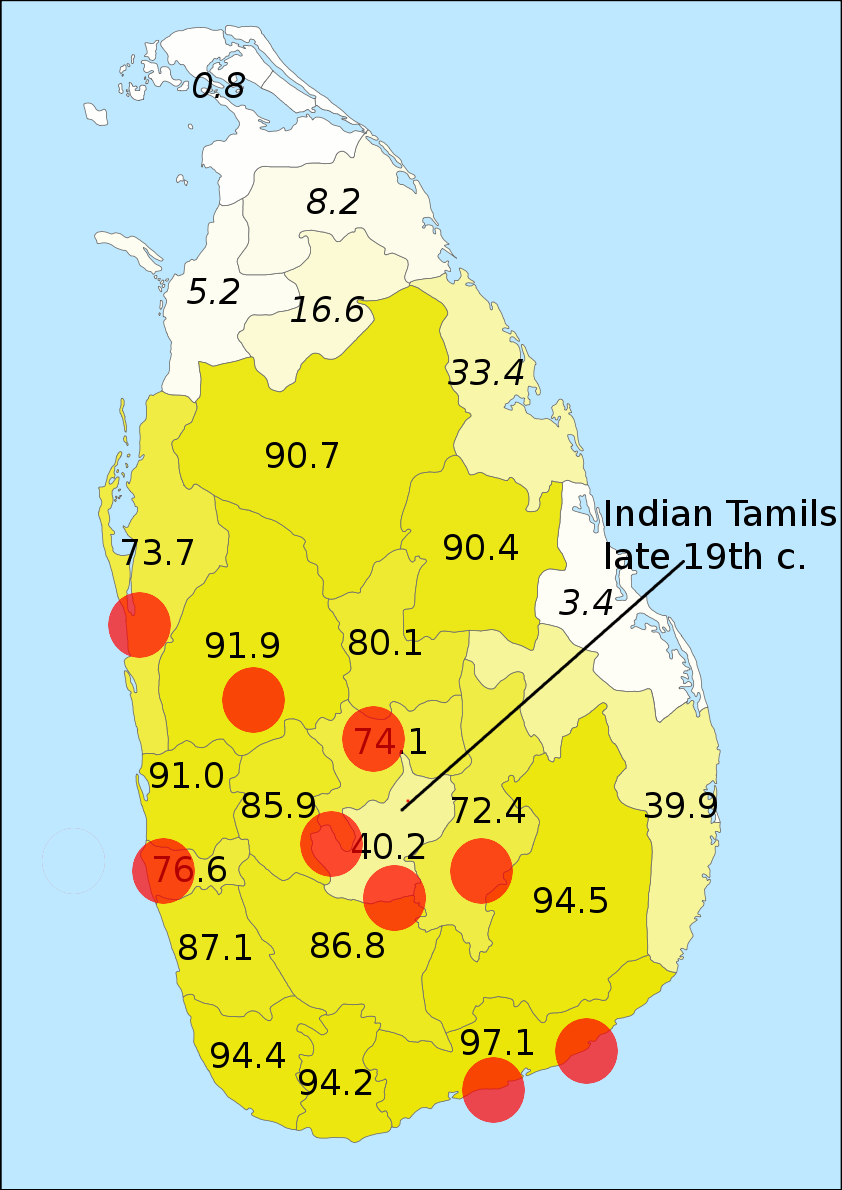
\includegraphics[width=.45\textwidth]{SriLankaSinhalese}
%  % SriLankaSinhalese.png: 0x0 pixel, 0dpi, 0.00x0.00 cm, bb=
% }
% \subfigure[Distribution of the Moor population]{
%  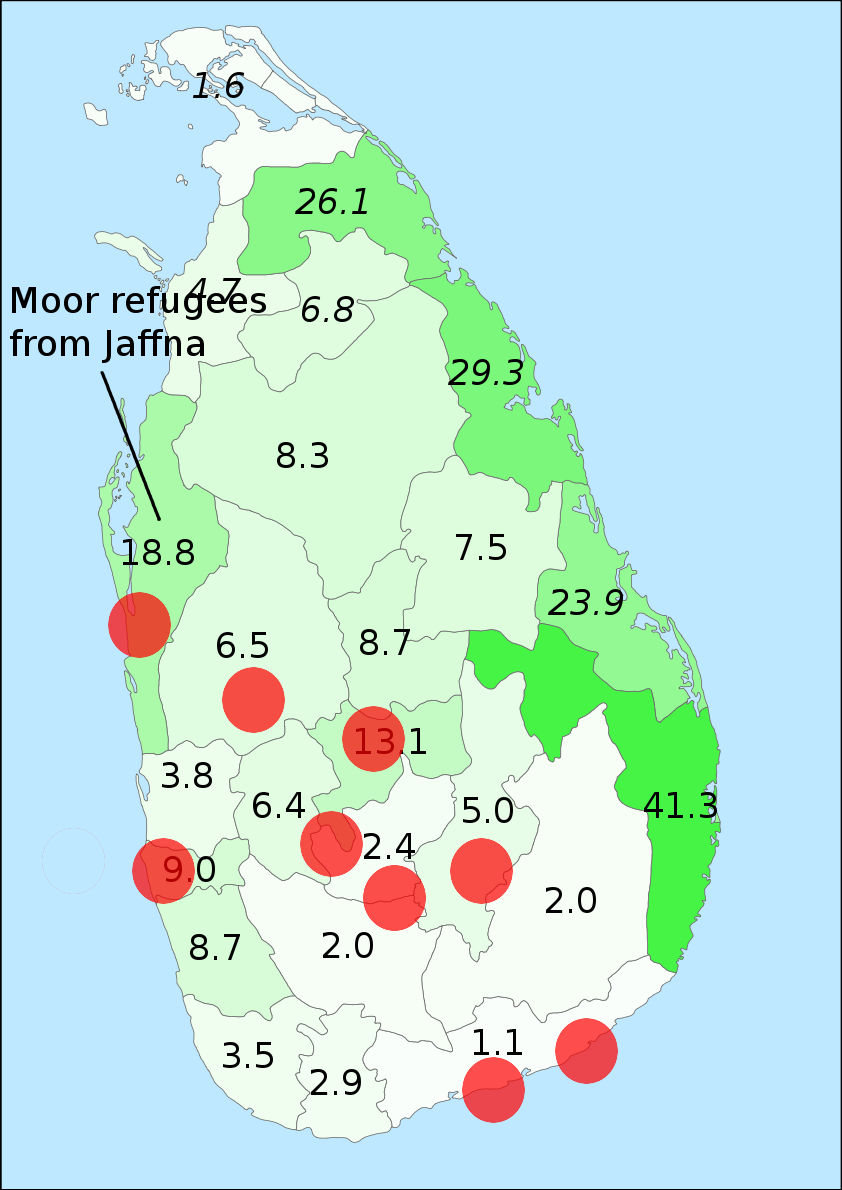
\includegraphics[width=.45\textwidth]{SriLankaMoor}
%  % SriLankaSinhalese.png: 0x0 pixel, 0dpi, 0.00x0.00 cm, bb=
%  }
%  \caption{Demographics of Sri Lanka. Dots mark main towns with Malay population. The Malay population centers are all in the Sinhala speaking area. Recent shifts in population leading to a skewed picture with regard to the early 19th century are indicated.}
% \end{sidewaysfigure}

\nocite{Verma1976,Gair1998}
\end{document}
